\documentclass{article}

\usepackage{amsmath, amsthm, amssymb, amsfonts, physics}
\usepackage{thmtools}
\usepackage{graphicx}
\usepackage{setspace}
\usepackage{geometry}
\usepackage{float}
\usepackage{hyperref}
\usepackage[utf8]{inputenc}
\usepackage[english]{babel}
\usepackage{framed}
\usepackage[dvipsnames]{xcolor}
\usepackage{tcolorbox}
\usepackage{ctex}
\usepackage{tikz-cd}
\usepackage{mathtools}
\usepackage[natbibapa]{apacite}
\usepackage{tabularray}
\usepackage{caption}
\usepackage{dcolumn}

\colorlet{LightGray}{White!90!Periwinkle}
\colorlet{LightOrange}{Orange!15}
\colorlet{LightGreen}{Green!15}
\colorlet{LightBlue}{Blue!15}

\newcommand{\HRule}[1]{\rule{\linewidth}{#1}}
\newcommand{\R}{\mathbb{R}}
\newcommand{\C}{\mathbb{C}}
\newcommand{\Q}{\mathbb{Q}}
\newcommand{\N}{\mathbb{N}}
\newcommand{\U}{\mathbb{U}}
\newcommand{\F}{\mathbb{F}}
\newcommand{\Hom}{\text{Hom}}
\newcommand{\id}{\text{Id}}
\newcommand{\Ker}{\text{Ker}}
\newcommand{\im}{\text{Im}}
\newcommand{\rk}{\text{rk}}
\newcommand{\mini}{\fontsize{8}{10}\selectfont}

\declaretheoremstyle[name=Theorem,]{thmsty}
\declaretheorem[style=thmsty,numberwithin=section]{theorem}
\tcolorboxenvironment{theorem}{colback=LightGreen}

\declaretheoremstyle[name=Proposition,]{prosty}
\declaretheorem[style=prosty,numberwithin=section]{proposition}
\tcolorboxenvironment{proposition}{colback=LightGray}

\declaretheoremstyle[name=Lemma,]{lemsty}
\declaretheorem[style=lemsty,numberwithin=section]{lemma}
\tcolorboxenvironment{lemma}{colback=LightOrange}

\declaretheoremstyle[name=Definition,]{defnsty}
\declaretheorem[style=defnsty,numberwithin=section]{definition}
\tcolorboxenvironment{definition}{colback=LightBlue}

\setstretch{1.2}
\geometry{
    textheight=9in,
    textwidth=5.5in,
    top=1in,
    headheight=12pt,
    headsep=25pt,
    footskip=30pt
}

\begin{document}

\title{ \normalsize \textsc{}
		\\ [2.0cm]
		\HRule{1.5pt} \\
		\LARGE \textbf{\uppercase{ECON 301 - Intermediate Microeconomic Analysis}
		\HRule{2.0pt} \\ [0.6cm] \LARGE{进阶微观经济学分析} \vspace*{10\baselineskip}}
		}
\date{}
\author{\textbf{Author} \\ 
		Wenyou (Tobias) Tian \\
        田文友 \\
		University of British Columbia \\
        英属哥伦比亚大学 \\
		2024}

\maketitle
\newpage

\tableofcontents
\newpage
\section{Introduction}
In April 2022, after the Okanagan campus of the University of British Columbia implemented an all-access dining system for their students, the Vancouver campus announced that it will also adopt a similar strategy for dining halls located in primarity first-year residences to promote food security and reduce waste \citep{introduce_all_access}. This dining plan allow students with meal plans to swipe their student card once and enjoy all types of food instead of paying for individual items \citep{ubcallaccessdining}. Students who have not signed up for a meal plan may also access the dining halls by paying between $\$$12 to $\$$20 before tax for a meal depending on the dining hours \citep{ubcallaccessdining}. The food service at UBC Vancouver suggests that this move helps to reduce food waste because food items are served in limited portions and students are encouraged to take multiple trips if they do not feel fulfilled \citep{ubcallaccessdining}. It is believed that this can prevent students from taking too much food all at once which may eventually be dumped because students overestimate their appetite.

According the sustainability goal set by UBC, reducing food waste helps to build a more sustainable food system that ensures local food security. Furthermore, as UBC invests more and more in the effort to recycle, reducing food waste also decreases the strain on recycling in general, where the same resource can be used to recycle other items.

Given this environmental initiative, this paper aims to investigate if the all-access dining plan introduced at the UBC Vancouver campus aligns with this sustainability goal of reducing food waste. Specifically, this paper hopes to unfold the relationship between the number of diners and the amount of food waste generated each day. With the data provided by UBC food service, it is possible to answer the question - \textbf{how does the number of diners of different dining hours impact the amount of food waste generated within each day across three food service facilities?} Here the facilities refer to the cafeteria located in the first-year residences, which are Totem Park (\textit{abbr. TP}), Orchard Commons (\textit{abbr. OC}), and Place Vanier (\textit{abbr. PV}). The provided dataset can answer this question as it includes all the food waste data and diners at each location at different hours for the first semester of the 2023-2024 school year.

Although the dataset suffers from heteroskedasticity, it is still hypothesized that for all three locations, the number of diners during at least one dining hours will have an impact on the amount of food waste generated in each day. However, \textbf{this paper concludes that} for the dining halls at Totem Park and Place Vanier, the number of diners have little to no impact on the food waste produced at these locations, while at Orchard Commons, the number of breakfast diners is negatively correlated with the amount of food waste and the number of lunch diners is positively correlated with the amount of food waste across days.

Given this conclusion, it is recommended that further measures can be taken to reduce food waste focusing on the dinner plates at Place Vanier and on lunch plates at Orchard Commons.
\newpage
\section{Data Description}
In the dataset provided by the UBC Food Service, it mainly consists of two types of data \citep{food_waste}. The first of which compiles all the menu option on the days that dining halls are accessible to students, and the second of which offers the data on the number of diners and the amount of food waste generated from preparation to consumption across different dining hours at three dining halls. Since the focus is to determine the relationship between the number of diners and the amount of food waste, the first type of data is mostly irrelevant to the question of interest. However, it should be mentioned that the dining halls rotate their menu options, thus, one of the assumptions made for this research is that \textbf{diners generally have consistent preferences so that leftovers are primarily generated by students unable to finish the dish rather than disliking the taste.}

Within the relevant dataset, which is the second type, there are several key issues to be resolved. 

The first one occurs in the recorded food waste data. It can be observed across all three dining halls, there are days where part of the process is missing a record, or during some days, it appears that the dinner hours included the previous hours whereas these hours are missing their data. Thus, a decision is made to only focus on all the waste generated within each day, disregarding specific processes and specific dining hours to account for missing records and unreasonable entries resulted from whatever reasons.

The second one occurs in the recorded diner numbers. It is also observed that there are days where the number of diners are not recorded for the specific dining hour. As it is critical for this research to look for the relationship across each dining hour, any data entry with at least one of the dining hours missing diner numbers is eliminated from the final summarized table.

After these selections, there are $89$ reasonable observations recorded at Totem Park, $96$ observations recorded at Orchard Commons, and $85$ observations recorded at Place Vanier. Each of the processed tables consists of the date of entry, the dining hall location, the number of diners for each dining hour, the total number of diners in a day, and the total waste in a day. The graphs of these relevant information is included in the Appendix.

\subsection{Summary Statistics Table}
To generally describe these processed data, a summary statistics table is included to provide basic interpretations of the variables. The relevant statistics include the mean, the standard deviation, and the maximum values of each data column in the table. Some general characteristics include: across all three locations, there are generally more lunch diners and dinner diners than breakfast diners; Orchard Commons appears to be a more popular choice for students than the other two locations; the average food waste across all three locations are between $300$ and $400$ units.

\begin{table}
    \captionsetup{justification=justified,singlelinecheck=false,margin=0pt}
    \caption{Mean, Standard Deviation and Maximum for Relevant Data Columns across Dining Halls}
    \centering
    \mini
    \begin{tblr}{
      cell{1}{1} = {c=2}{},
      cell{2}{1} = {r=3}{},
      cell{5}{1} = {r=3}{},
      cell{8}{1} = {r=3}{},
      vlines,
      hline{1-2,5,8,11} = {-}{},
      hline{3-4,6-7,9-10} = {2-7}{},
    }
                    &      & Breakfast & Lunch     & Dinner    & Diner Total & Waste Total \\
    Totem Park      & Mean & 693.2022  & 1018.7416 & 1109.8539 & 2821.7978   & 399.3076    \\
                    & SD   & 386.6350  & 248.6930  & 388.3880  & 524.6679    & 344.7666    \\
                    & Max  & 1797.00   & 1806.00   & 1884.00   & 3694.00     & 3208.01     \\
    Orchard Commons & Mean & 753.4167  & 1292.0625 & 1456.3333 & 3501.8125   & 314.0145    \\
                    & SD   & 279.6764  & 329.5889  & 342.0098  & 884.5424    & 127.8332    \\
                    & Max  & 1298.00   & 1794.00   & 2093.00   & 4496.00     & 740.68      \\
    Place Vanier    & Mean & 739.8235  & 1014.8824 & 910.0824  & 2664.7882   & 396.0318    \\
                    & SD   & 344.5338  & 327.6320  & 353.1179  & 731.2697    & 241.4976    \\
                    & Max  & 1372.00   & 1513.00   & 1468.00   & 3650.00     & 1659.90
    \end{tblr} \\
    \medskip
    \normalsize
    \raggedright The unit for food waste is never clarified by the data provider, it is assumed that the food waste is measured in pounds (lb).
\end{table}
\section{Model}
Reiterating the goal of this paper, it investigates the impact of the number of diners of each dining hour on the amount of food waste generated with each day. After the selection of data, the table consists of the relevant variables for each dining location. Apart from the aforementioned assumption made, two more assumptions are made to set up this model.
\begin{quote}
    1. It is assumed that the food waste is primarily generated due to the number of diners. This assumption is made based upon how the waste data is categorized. Since the waste data breaks down the waste into different preparation and consumption stages, it is assumed that an increase in the number of diners would lead to an increase in waste during preparation stages as well. \\
    2. It is assumed that the number of diners across the semester is consistent and random, where the number of diners on one day is not affected by the day before and dining halls do not suffer significant increases and drops. This assumption incorporates three phenomena in the students. First, the students may go to other cafeterias as there is no restriction on which dining hall students can access. Second, most students go to the dining halls most closely located to their dormitories. Third, students may also choose to skip certain meals due to their timetables.
\end{quote}
Given the goal of the paper and these assumptions, it is possible to set up the following multiple linear regression to answer the research question:
$$W_i = \beta_0 + \beta_1 B_i + \beta_2 L_i + \beta_3 S_i + \epsilon_i$$
The relevant variables are labeled as follows:
\begin{quote}
    1. $W_i$: the total amount of food waste generated on the $i$th day in the dataset, it is assumed that this is measured in pounds (lb). \\
    2. $B_i$: the number of breakfast diners on the $i$th day. \\
    3. $L_i$: the number of lunch diners on the $i$th day. \\
    4. $S_i$: the number of dinner diners on the $i$th day.
\end{quote}
Notice that the same regression model will be applied to each of the dining halls to observer the effect.

By the setup of this regression, $\beta_1$ represents the change in daily food waste subject to $1$-unit increase in the breakfast diners, $\beta_2$ represents the change in daily food waste subject to $1$-unit increase in the lunch diners, and $\beta_3$ is a similar parameter for $1$-unit increase in the dinner diners. Here $\beta_0$ plays the role of representing all the food waste generated by all other sources apart from the number of diners.

\subsection{Specifications}
The main specification from this regression model investigates if the number of diners of at least one dining hour has an impact on the daily food waste. This is characterized by investigating if all the parametric coefficients of the number of diners is $0$. Thus, we set up the main null hypothesis:
$$H_0^{(0)}: \beta_1 = \beta_2 = \beta_3 = 0$$
Three other specifications are also introduced. The main specification only answers if there is an impact, but does not answer which dining hour actually contributes to this consequence. Therefore, it is also motivated to investigate if the parametric coefficients have an impact on the daily food waste independently. Thus, we can set up three more null hypotheses:
$$H_0^{(1)}: \beta_1 = 0$$
$$H_0^{(2)}: \beta_2 = 0$$
$$H_0^{(3)}: \beta_3 = 0$$
To test the robustness of this model, that is, if the variables are grouped differently, would there be a change on the conclusion reached. In this case, it is possible to set up another simple linear regression:
$$W_i = \alpha_0 + \alpha_1 C_i + \eta_i$$
where $W_i$ represents the same thing, but $C_i$ represents the total number of diners on the $i$th day.

Here, it is possible to test if the total diners have an impact on the food waste as well, aligning with the research question. Thus, the null hypothesis for this can be set up as:
$$H_0^{'}: \alpha_1 = 0$$

\newpage
\section{Table of Results}

% Table created by stargazer v.5.2.3 by Marek Hlavac, Social Policy Institute. E-mail: marek.hlavac at gmail.com
% Date and time: Sun, Apr 21, 2024 - 10:07:20 PM
% Requires LaTeX packages: dcolumn 
\begin{table}[!htbp] \centering 
  \caption{Totem Park: Effect of Number of People Dining on Food Waste} 
  \label{} 
\begin{tabular}{@{\extracolsep{5pt}}lD{.}{.}{-3} D{.}{.}{-3} D{.}{.}{-3} D{.}{.}{-3} } 
\\[-1.8ex]\hline 
\hline \\[-1.8ex] 
 & \multicolumn{4}{c}{\textit{Dependent variable:}} \\ 
\cline{2-5} 
\\[-1.8ex] & \multicolumn{4}{c}{Waste\_Total} \\ 
\\[-1.8ex] & \multicolumn{1}{c}{(1)} & \multicolumn{1}{c}{(2)} & \multicolumn{1}{c}{(3)} & \multicolumn{1}{c}{(4)}\\ 
\hline \\[-1.8ex] 
 Breakfast & 0.178^{*} &  &  & 0.162 \\ 
  & (0.094) &  &  & (0.099) \\ 
  & & & & \\ 
 Lunch &  & -0.022 &  & -0.051 \\ 
  &  & (0.149) &  & (0.148) \\ 
  & & & & \\ 
 Dinner &  &  & -0.109 & -0.063 \\ 
  &  &  & (0.094) & (0.099) \\ 
  & & & & \\ 
 Constant & 275.614^{***} & 421.291^{***} & 520.606^{***} & 408.636^{*} \\ 
  & (74.248) & (155.792) & (110.986) & (212.669) \\ 
  & & & & \\ 
\hline \\[-1.8ex] 
Observations & \multicolumn{1}{c}{89} & \multicolumn{1}{c}{89} & \multicolumn{1}{c}{89} & \multicolumn{1}{c}{89} \\ 
R$^{2}$ & \multicolumn{1}{c}{0.040} & \multicolumn{1}{c}{0.0002} & \multicolumn{1}{c}{0.015} & \multicolumn{1}{c}{0.046} \\ 
\hline 
\hline \\[-1.8ex] 
\textit{Note:}  & \multicolumn{4}{r}{$^{*}$p$<$0.1; $^{**}$p$<$0.05; $^{***}$p$<$0.01} \\ 
\end{tabular} 
\end{table} 


% Table created by stargazer v.5.2.3 by Marek Hlavac, Social Policy Institute. E-mail: marek.hlavac at gmail.com
% Date and time: Sun, Apr 21, 2024 - 10:07:21 PM
% Requires LaTeX packages: dcolumn 
\begin{table}[!htbp] \centering 
  \caption{Orchard Commons: Effect of Number of People Dining on Food Waste} 
  \label{} 
\begin{tabular}{@{\extracolsep{5pt}}lD{.}{.}{-3} D{.}{.}{-3} D{.}{.}{-3} D{.}{.}{-3} } 
\\[-1.8ex]\hline 
\hline \\[-1.8ex] 
 & \multicolumn{4}{c}{\textit{Dependent variable:}} \\ 
\cline{2-5} 
\\[-1.8ex] & \multicolumn{4}{c}{Waste\_Total} \\ 
\\[-1.8ex] & \multicolumn{1}{c}{(1)} & \multicolumn{1}{c}{(2)} & \multicolumn{1}{c}{(3)} & \multicolumn{1}{c}{(4)}\\ 
\hline \\[-1.8ex] 
 Breakfast & 0.126^{***} &  &  & -0.254^{***} \\ 
  & (0.045) &  &  & (0.077) \\ 
  & & & & \\ 
 Lunch &  & 0.192^{***} &  & 0.373^{***} \\ 
  &  & (0.035) &  & (0.072) \\ 
  & & & & \\ 
 Dinner &  &  & 0.135^{***} & 0.005 \\ 
  &  &  & (0.036) & (0.054) \\ 
  & & & & \\ 
 Constant & 218.734^{***} & 65.914 & 116.879^{**} & 16.681 \\ 
  & (36.385) & (46.333) & (53.742) & (52.236) \\ 
  & & & & \\ 
\hline \\[-1.8ex] 
Observations & \multicolumn{1}{c}{96} & \multicolumn{1}{c}{96} & \multicolumn{1}{c}{96} & \multicolumn{1}{c}{96} \\ 
R$^{2}$ & \multicolumn{1}{c}{0.077} & \multicolumn{1}{c}{0.245} & \multicolumn{1}{c}{0.131} & \multicolumn{1}{c}{0.327} \\ 
\hline 
\hline \\[-1.8ex] 
\textit{Note:}  & \multicolumn{4}{r}{$^{*}$p$<$0.1; $^{**}$p$<$0.05; $^{***}$p$<$0.01} \\ 
\end{tabular} 
\end{table} 


% Table created by stargazer v.5.2.3 by Marek Hlavac, Social Policy Institute. E-mail: marek.hlavac at gmail.com
% Date and time: Sun, Apr 21, 2024 - 10:07:22 PM
% Requires LaTeX packages: dcolumn 
\begin{table}[!htbp] \centering 
  \caption{Place Vanier: Effect of Number of People Dining on Food Waste} 
  \label{} 
\begin{tabular}{@{\extracolsep{5pt}}lD{.}{.}{-3} D{.}{.}{-3} D{.}{.}{-3} D{.}{.}{-3} } 
\\[-1.8ex]\hline 
\hline \\[-1.8ex] 
 & \multicolumn{4}{c}{\textit{Dependent variable:}} \\ 
\cline{2-5} 
\\[-1.8ex] & \multicolumn{4}{c}{Waste\_Total} \\ 
\\[-1.8ex] & \multicolumn{1}{c}{(1)} & \multicolumn{1}{c}{(2)} & \multicolumn{1}{c}{(3)} & \multicolumn{1}{c}{(4)}\\ 
\hline \\[-1.8ex] 
 Breakfast & 0.045 &  &  & 0.088 \\ 
  & (0.077) &  &  & (0.091) \\ 
  & & & & \\ 
 Lunch &  & 0.071 &  & -0.062 \\ 
  &  & (0.081) &  & (0.107) \\ 
  & & & & \\ 
 Dinner &  &  & 0.149^{**} & 0.183^{**} \\ 
  &  &  & (0.073) & (0.090) \\ 
  & & & & \\ 
 Constant & 362.526^{***} & 324.438^{***} & 260.400^{***} & 226.471^{**} \\ 
  & (62.593) & (85.840) & (71.464) & (98.692) \\ 
  & & & & \\ 
\hline \\[-1.8ex] 
Observations & \multicolumn{1}{c}{85} & \multicolumn{1}{c}{85} & \multicolumn{1}{c}{85} & \multicolumn{1}{c}{85} \\ 
R$^{2}$ & \multicolumn{1}{c}{0.004} & \multicolumn{1}{c}{0.009} & \multicolumn{1}{c}{0.047} & \multicolumn{1}{c}{0.059} \\ 
\hline 
\hline \\[-1.8ex] 
\textit{Note:}  & \multicolumn{4}{r}{$^{*}$p$<$0.1; $^{**}$p$<$0.05; $^{***}$p$<$0.01} \\ 
\end{tabular} 
\end{table} 

For each table, the first column is regressed between the total daily waste and \textbf{only} the number of breakfast diners, the second and third column follows a similar suit where they are regressed \textbf{only} the number of lunch diners and dinner diners respectively.
\section{Discussion}
Before reporting any useful conclusions, possible issues in the regression model need to be addressed first. In the graph presented in the Appendix, it is likely that the explanatory variables in the regression model suffer from heteroskedasticity. Therefore, White's test is performed for all three multiple regressions first.

It yields that all three regressions failed the White's test, thus, it is necessary not to assume homoskedasticity, and compute the robust standard errors for these explanatory variables. In this case, by incorporating the robust standard errors, the regression tables are presented as the following with comparisons made when homoskedasticity is assumed, the errors for the variables have now been adjusted to incorporate heteroskedasticity:

% Table created by stargazer v.5.2.3 by Marek Hlavac, Social Policy Institute. E-mail: marek.hlavac at gmail.com
% Date and time: Sun, Apr 21, 2024 - 10:07:24 PM
% Requires LaTeX packages: dcolumn 
\begin{table} \centering 
  \caption{Totem Park: Robust Standard Error Incorporation} 
  \label{} 
\begin{tabular}{@{\extracolsep{5pt}}lD{.}{.}{-3} D{.}{.}{-3} } 
\\[-1.8ex]\hline 
\hline \\[-1.8ex] 
 & \multicolumn{2}{c}{\textit{Dependent variable:}} \\ 
\cline{2-3} 
\\[-1.8ex] & \multicolumn{2}{c}{Waste\_Total} \\ 
 & \multicolumn{1}{c}{default} & \multicolumn{1}{c}{robust} \\ 
\\[-1.8ex] & \multicolumn{1}{c}{(1)} & \multicolumn{1}{c}{(2)}\\ 
\hline \\[-1.8ex] 
 Breakfast & 0.162 & 0.162^{*} \\ 
  & (0.099) & (0.085) \\ 
  & & \\ 
 Lunch & -0.051 & -0.051 \\ 
  & (0.148) & (0.076) \\ 
  & & \\ 
 Dinner & -0.063 & -0.063 \\ 
  & (0.099) & (0.133) \\ 
  & & \\ 
 Constant & 408.636^{*} & 408.636^{**} \\ 
  & (212.669) & (205.983) \\ 
  & & \\ 
\hline \\[-1.8ex] 
Observations & \multicolumn{1}{c}{89} & \multicolumn{1}{c}{89} \\ 
R$^{2}$ & \multicolumn{1}{c}{0.046} & \multicolumn{1}{c}{0.046} \\ 
\hline 
\hline \\[-1.8ex] 
\textit{Note:}  & \multicolumn{2}{r}{$^{*}$p$<$0.1; $^{**}$p$<$0.05; $^{***}$p$<$0.01} \\ 
\end{tabular} 
\end{table} 


% Table created by stargazer v.5.2.3 by Marek Hlavac, Social Policy Institute. E-mail: marek.hlavac at gmail.com
% Date and time: Sun, Apr 21, 2024 - 10:07:25 PM
% Requires LaTeX packages: dcolumn 
\begin{table} \centering 
  \caption{Orchard Commons: Robust Standard Error Incorporation} 
  \label{} 
\begin{tabular}{@{\extracolsep{5pt}}lD{.}{.}{-3} D{.}{.}{-3} } 
\\[-1.8ex]\hline 
\hline \\[-1.8ex] 
 & \multicolumn{2}{c}{\textit{Dependent variable:}} \\ 
\cline{2-3} 
\\[-1.8ex] & \multicolumn{2}{c}{Waste\_Total} \\ 
 & \multicolumn{1}{c}{default} & \multicolumn{1}{c}{robust} \\ 
\\[-1.8ex] & \multicolumn{1}{c}{(1)} & \multicolumn{1}{c}{(2)}\\ 
\hline \\[-1.8ex] 
 Breakfast & -0.254^{***} & -0.254^{***} \\ 
  & (0.077) & (0.096) \\ 
  & & \\ 
 Lunch & 0.373^{***} & 0.373^{***} \\ 
  & (0.072) & (0.097) \\ 
  & & \\ 
 Dinner & 0.005 & 0.005 \\ 
  & (0.054) & (0.054) \\ 
  & & \\ 
 Constant & 16.681 & 16.681 \\ 
  & (52.236) & (47.548) \\ 
  & & \\ 
\hline \\[-1.8ex] 
Observations & \multicolumn{1}{c}{96} & \multicolumn{1}{c}{96} \\ 
R$^{2}$ & \multicolumn{1}{c}{0.327} & \multicolumn{1}{c}{0.327} \\ 
\hline 
\hline \\[-1.8ex] 
\textit{Note:}  & \multicolumn{2}{r}{$^{*}$p$<$0.1; $^{**}$p$<$0.05; $^{***}$p$<$0.01} \\ 
\end{tabular} 
\end{table} 
 

% Table created by stargazer v.5.2.3 by Marek Hlavac, Social Policy Institute. E-mail: marek.hlavac at gmail.com
% Date and time: Sun, Apr 21, 2024 - 10:07:26 PM
% Requires LaTeX packages: dcolumn 
\begin{table} \centering 
  \caption{Place Vanier: Robust Standard Error Incorporation} 
  \label{} 
\begin{tabular}{@{\extracolsep{5pt}}lD{.}{.}{-3} D{.}{.}{-3} } 
\\[-1.8ex]\hline 
\hline \\[-1.8ex] 
 & \multicolumn{2}{c}{\textit{Dependent variable:}} \\ 
\cline{2-3} 
\\[-1.8ex] & \multicolumn{2}{c}{Waste\_Total} \\ 
 & \multicolumn{1}{c}{default} & \multicolumn{1}{c}{robust} \\ 
\\[-1.8ex] & \multicolumn{1}{c}{(1)} & \multicolumn{1}{c}{(2)}\\ 
\hline \\[-1.8ex] 
 Breakfast & 0.088 & 0.088 \\ 
  & (0.091) & (0.079) \\ 
  & & \\ 
 Lunch & -0.062 & -0.062 \\ 
  & (0.107) & (0.096) \\ 
  & & \\ 
 Dinner & 0.183^{**} & 0.183^{*} \\ 
  & (0.090) & (0.102) \\ 
  & & \\ 
 Constant & 226.471^{**} & 226.471^{***} \\ 
  & (98.692) & (83.577) \\ 
  & & \\ 
\hline \\[-1.8ex] 
Observations & \multicolumn{1}{c}{85} & \multicolumn{1}{c}{85} \\ 
R$^{2}$ & \multicolumn{1}{c}{0.059} & \multicolumn{1}{c}{0.059} \\ 
\hline 
\hline \\[-1.8ex] 
\textit{Note:}  & \multicolumn{2}{r}{$^{*}$p$<$0.1; $^{**}$p$<$0.05; $^{***}$p$<$0.01} \\ 
\end{tabular} 
\end{table} 

\newpage

\subsection{Specification Check}
For each dining hall, tests for $H_0^{(0)}, H_0^{(1)}, H_0^{(2)}, H_0^{(3)}$ are performed to see if the result presented in the above regression table answers the research question.

For the Totem Park dining hall, one fails to reject all four null hypotheses. This indicates that it is statistically possible for none of the number of diners to have any impact on the food waste. Even if an additional null hypothesis $H_0^{4}: \beta_0 = 0$ is tested, the test yields $p \approx 0.058 < 0.06$, indicating there is still about a $6\%$ chance that the null hypothesis is true. Thus, it can be asserted that the parameters in Totem Park's regression table are statistically insignificant.

For the Orchard Commons dining hall, one only fails to reject $H_0^{3}$, that is in the multiple regression, it is possible for the number of dinner diners to have no impact on the daily food waste. Therefore, it can be concluded that the number of diners of at least one dining hour has an impact on the daily waste where, specifically, it is the breakfast diners and lunch diners who contribute to this impact. By analyzing Orchard Commons' regression table, the parameters read $\beta_2 = -0.254 \pm 0.096$ and $\beta_3 = 0.373 \pm 0.097$. It can interpreted that for an extra unit of breakfast diners, the daily food waste is expected to decrease by about $-0.25$ pounds; whereas for an extra unit of lunch diners, the daily food waste is expected to increase by about $0.37$ pounds. Thus, apart from the number of diners, it is possible for other factors to explain this difference between dining hours.

For the Place Vanier dining hall, one fails to reject these null hypotheses: $H_0^{(1)}$, and $H_0^{(2)}$. However, for the test on $H_0^{(0)}$, it yields that $p \approx 0.06 < 0.1$, and for the test on $H_0^{(3)}$, it yields that $p \approx 0.04 < 0.05$. From this, a weak conclusion can be made: if the number of diners indeed has an impact on the amount of daily food waste, the source of such an impact is most likely to be the number of dinner diners at Place Vanier. The regression table reported that for the dinner diners, the parameter reads $\beta_3 = 0.183 \pm 0.102$, indicating for an extra unit of dinner diners, it is expected that the daily food waste to increase by about $0.18$ units. Similar to Orchard Commons' situation, other factors can be incorporated to discuss why this is the case.

\subsection{Robustness Analysis}
Alongside the multiple regression model, the other aforementioned simple regression on the relationship between the amount of daily food waste and the total number of diners is also performed to compare if the results concluded from the previous section are consistent.

For Totem Park, the non-robust result from this regression yields $\alpha_1 = 0.032 \pm 0.070$. The null hypothesis states that $H_0^{'}: \alpha_1 = 0$, and the test for this specification yields that it fails to reject the null hypothesis, indicating it is highly possible that the number of diners has no impact on the amount of daily food waste. This indication aligns with what is concluded in the previous section.

For Orchard Commons, the non-robust result from the regression yields $\alpha_1 = 0.060 \pm 0.014$ and the test for the null hypothesis rejects the null hypothesis by a wide margin. This indicates if one considers all diners at Orchard Commons as a whole, for an extra unit of diner, it is expected that the daily food waste will increase by about $0.06$ pounds. This indeed aligns with what is concluded in the previous section, where the number of diners does have impact on the daily food waste. This regression suggests that the impact from each dining hour is evened out.

For Place Vanier, the non-robust result from the regression yields $\alpha_1 = 0.059 \pm 0.036$ and the test yields that one fails to reject the null hypothesis. There is more than $10\%$ chance that the null hypothesis is factually true. This still somewhat aligns with the results reached from the previous section. The previous section concludes that if there is an impact from the number of diners on the amount of daily food waste, the impact is most likely sourced from the number of dinner diners. The current regression can further affirm that the effect of the number of dinner diners may be masked by the diners at other dining hours, since as a whole, it is still very likely that there is no impact from the number of diners at all.

\subsection{Summary}
In this \textbf{\textit{Discussion}} section, it is first demonstrated that the explanatory variables suffer from heteroskedasticity.

By comparing and contrasting the conclusions made from both specification checks and robustness tests, it is seen that the same conclusions can be reached and the results align with each other with proper reasoning.

\newpage
\section{Conclusion}
The paper aims to investigate whether the switch from pay-per-item at dining halls to all-access-dining by UBC Vancouver campus has contributed to reducing food waste or not. The major question this paper hopes to answer is that how the number of diners of different dining hours contribute to the total daily food waste across three dining halls.

Certain data entries are eliminated during the process because they are missing records of data which may influence the result of the analysis. A multiple linear regression is set up to correlate the daily food waste and the number of diners during each dining hour, where the main specification is to determine whether or not the number of diners in at least one dining hour has an impact on the amount of daily food waste. Other relevant specifications investigate if the number of diners in each dining hour has an impact on the food waste. Another simple linear regression is set up to compare and contrast whether the results obtained from the multiple regression are consistent or not.

Since the explanatory variables suffer from heteroskedasticity, a robust standard error is incorporated. For Totem Park, it is concluded that the number of diners of any dining hour has little to no impact on the daily food waste. For Orchard Commons, it is summarized that the number of breakfast diners is negatively correlated with the amount of daily waste whereas the number of lunch diners is positively correlated with the amount of daily waste. For Place Vanier, it is unclear that as a whole, whether or not the number of diners has an impact on the daily waste, but if there is an impact, the most likely source is the number of dinner diners which is positively correlated with the amount of food waste.

The writer thus recommends for further investigation, other factors should be incorporated to explain the difference between the breakfast diners and lunch diners at Orchard Commons. More data is probably required to reach a more solid conclusion for Place Vanier, whereas for Totem Park, it is recommended to find reasons other than the number of diners to explain the food waste.

\bigskip
\textbf{Additional Note}: All data, figures (including those in the Appendix), tables are the result of the \textbf{\textit{Data Workbook}} \citep{data_workbook}. The \textbf{\textit{Data Workbook}} includes different R libraries utilized in the process of data analysis. The libraries usage is properly referenced in the workbook. Furthermore, the basic code to clean up the data involved is based on the file $\verb|cleanup.r|$, which is the work done by the ECON 326 teaching team \citep{cleanup}. The template for this paper is based on an Overleaf template published for public use \citep{template}.

\newpage

\bibliographystyle{apacite}
\bibliography{references.bib}

\newpage
\section{Appendix}
\begin{center}
    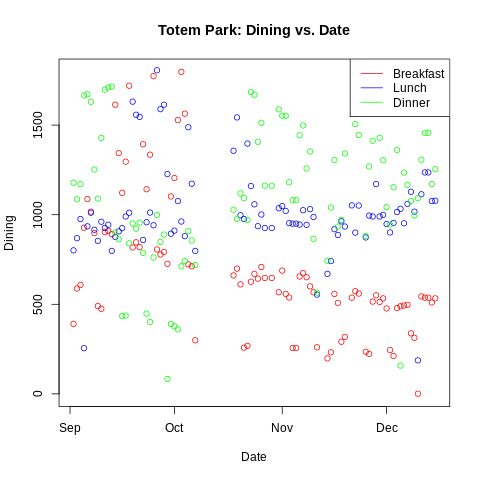
\includegraphics[scale = 0.575]{graph_table/TP_dining.png}
    \captionof{figure}{Totem Park: Number of Diners vs. Date}
\end{center}

\begin{center}
    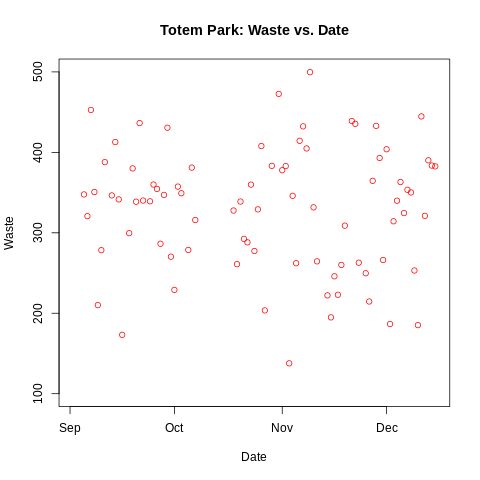
\includegraphics[scale = 0.575]{graph_table/TP_waste.png}
    \captionof{figure}{Totem Park: Daily Food Waste vs. Date}
\end{center}

\begin{center}
    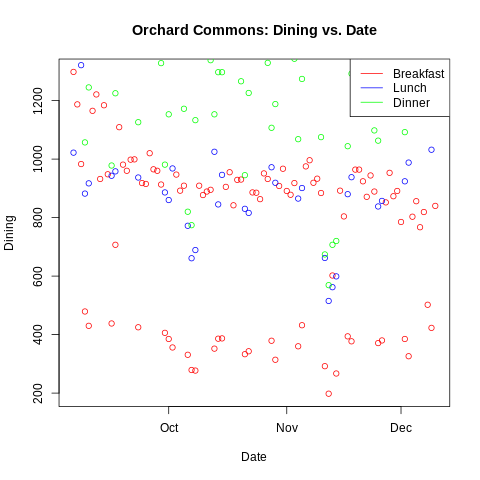
\includegraphics[scale = 0.575]{graph_table/OC_dining.png}
    \captionof{figure}{Orchard Commons: Number of Diners vs. Date}
\end{center}

\begin{center}
    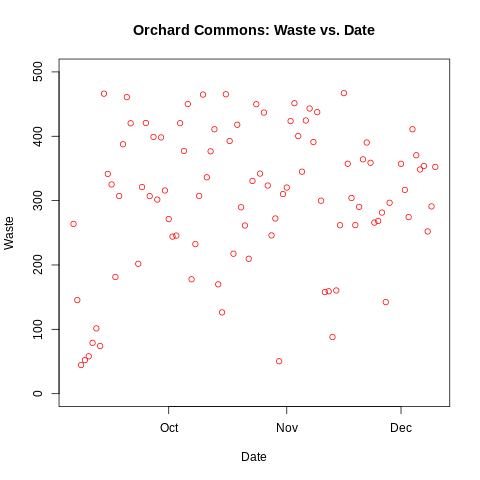
\includegraphics[scale = 0.575]{graph_table/OC_waste.png}
    \captionof{figure}{Orchard Commons: Daily Food Waste vs. Date}
\end{center}

\begin{center}
    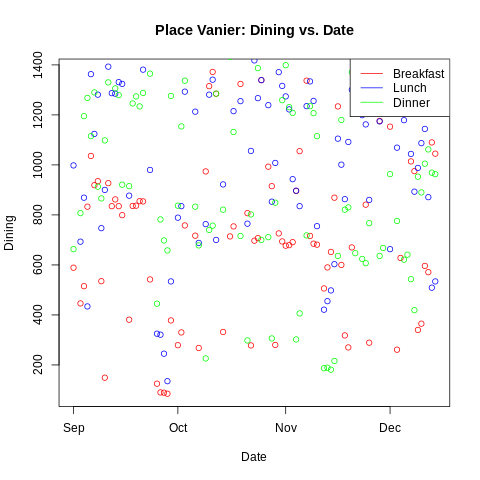
\includegraphics[scale = 0.575]{graph_table/PV_dining.png}
    \captionof{figure}{Place Vanier: Number of Diners vs. Date}
\end{center}

\begin{center}
    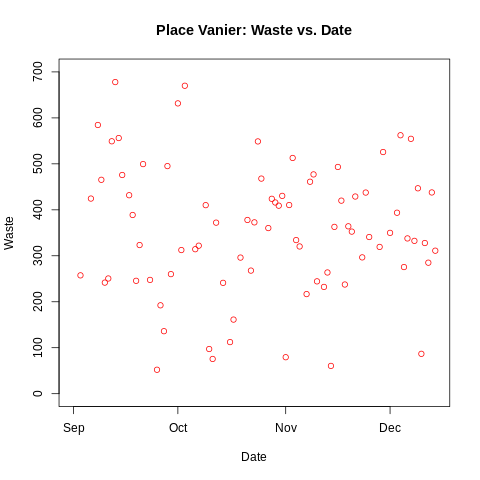
\includegraphics[scale = 0.575]{graph_table/PV_waste.png}
    \captionof{figure}{Place Vanier: Daily Food Waste vs. Date}
\end{center}

\end{document}